Explain our implementations.. views, controllers\\
strategy used for handling the results obtained from LOV catalogue

\begin{figure}[!bht]
\center
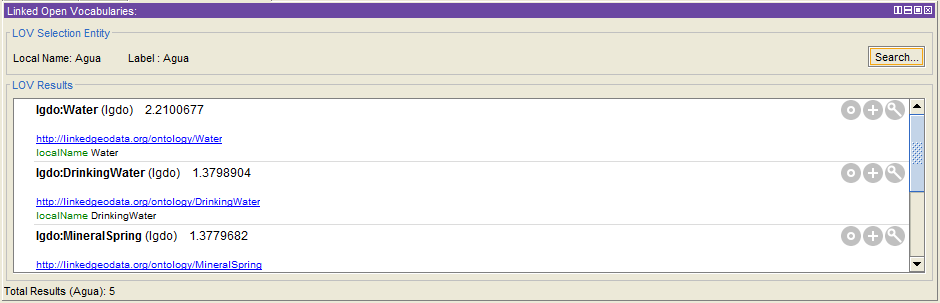
\includegraphics[scale=0.6]{img/LOVmockup.png}
\label{fig:LOVresults}
\caption{Panel showing the results for searching a term in the class hierarchy.}
\end{figure}


\begin{figure}[!bht]
\center
\includegraphics[scale=0.6]{img/LOVOptions.png}
\caption{Three actions currently available in the plugin after looking up a term in LOV catalogue: (a) reuse direct, (b) add equivalent axiom and (c) add subClass axiom}
\label{fig:LOVoptions}
\end{figure}
